\chapter{Subordination et coordination} \label{ch:subord-coord-fr}

\epigraph{If I were a cinnamon peeler\\
I would ride your bed\\
and leave the yellow bark dust\\
on your pillow.}{Michael Ondaatje, \enquote{The Cinnamon Peeler}}

\begin{tblsframedsymbol}{Objectifs d'apprentissage}{bulb}
\begin{itemize}[noitemsep, leftmargin=*]
    \item Distinguer la subordination, qui crée une dépendance hiérarchique, de la coordination, qui unit des éléments de statut égal.
    \item Identifier et analyser les propositions matrices, principales et subordonnées dans des phrases complexes.
    \item Reconnaître différents types de propositions subordonnées: propositions de contenu, propositions comparatives et propositions relatives.
    \item Comprendre que les subordonnants et les coordonnants fonctionnent comme des marqueurs structuraux plutôt que comme des têtes.
    \item Analyser les structures coordonnées, y compris la coordination de syntagmes et la coordination de propositions.
    \item Appliquer des tests diagnostiques pour déterminer les relations structurales dans des phrases complexes.
    \item Reconnaître comment la subordination et la coordination travaillent ensemble pour créer de la cohésion textuelle.
    \item Comprendre l'intérêt pédagogique de ces structures pour développer la conscience syntaxique.
\end{itemize}
\end{tblsframedsymbol}

\section{Introduction}

La langue nous permet d'exprimer non seulement des idées isolées, mais aussi les relations entre ces idées. Deux moyens fondamentaux pour le faire sont la \term{subordination} (angl. \term{subordination}) et la \term{coordination} (angl. \term{coordination}). Chacun a une fonction distincte: la subordination crée des hiérarchies de dépendance, tandis que la coordination unit des éléments de statut égal.

Considérez ces trois façons de relier les mêmes idées de base:

\ea \label{ex:intro-fr}
    \ea \gll Kim left. Pat came.\\
        Kim partir-PASSÉ Pat venir-PASSÉ\\
    \glt `Kim est partie. Pat est venu.' [séparées]
    \ex \gll The fact {\ob}that Kim left{\cb} enabled Pat's arrival.\\
        le fait Sdr Kim partir-PASSÉ permettre-PASSÉ arrivée de-Pat\\
    \glt `Le fait que Kim soit partie a permis l'arrivée de Pat.' [subordonnée]
    \ex \gll Kim left and Pat came.\\
        Kim partir-PASSÉ et Pat venir-PASSÉ\\
    \glt `Kim est partie et Pat est venu.' [coordonnée]
    \z
\z
Dans (\ref{ex:intro-fr}a), nous avons deux énoncés indépendants. Dans (b), \mention{that Kim left} est enchâssé dans une structure plus grande: il fonctionne comme complément dans le sujet. Dans (c), les deux propositions sont mises sur le même plan: elles se présentent comme égales, simplement reliées par \mention{and}.

Ce contraste entre hiérarchie et égalité est profond en grammaire. Quand nous subordonnons une proposition à une autre, nous créons une relation de dépendance: une proposition sert de complément ou de modificateur à un élément de l'autre. Quand nous coordonnons des éléments, nous affirmons leur statut égal dans la structure, même s'ils diffèrent par ailleurs.

Les outils utilisés pour ces différentes relations sont peu nombreux: des mots comme \mention{that} et \mention{whether} pour les relations de dépendance, et des mots comme \mention{and}, \mention{or} et \mention{but} pour les relations d'égalité. Pourtant, ces petits mots nous permettent de construire des significations complexes à partir de parties simples, de montrer comment les idées sont reliées et de guider notre public à travers de longues chaînes de raisonnement. Ces éléments signalent une relation grammaticale plutôt qu'ils ne servent de têtes.

Dans ce chapitre, nous verrons comment ces deux systèmes fonctionnent, séparément et ensemble. Nous verrons comment la subordination permet d'insérer une pensée dans une autre, en créant des couches de sens. Nous examinerons comment la coordination permet de construire des idées complexes tout en gardant une structure simple. Enfin, nous verrons comment ces deux systèmes se complètent et nous donnent la souplesse nécessaire pour exprimer presque n'importe quelle relation entre des idées.

\section{Subordination}\label{sec:subordination-fr}

Quand nous communiquons, nous devons souvent exprimer des relations complexes entre des idées. Parfois, une idée dépend d'une autre; parfois, une pensée sert à modifier ou à expliquer une autre pensée. C'est là qu'intervient la subordination. La \term{subordination} est le procédé grammatical par lequel nous faisons d'une proposition un \term{dépendant} (\term{dependent}) dans une autre structure.

Une proposition qui contient une \term{proposition subordonnée} (\term{subordinate clause}) est appelée \term{proposition matrice} (\term{matrix clause}); une proposition qui n'est pas contenue dans une matrice est appelée \term{proposition principale} (\term{main clause}). Une proposition peut être à la fois principale et matrice, comme le montre l'exemple suivant.

\ea \label{ex:sub-basic-fr}
    \ea \gll Kim left early.\\
        Kim partir-PASSÉ tôt\\
    \glt `Kim est partie tôt.' [principale]
    \ex \gll She thinks {[}that Kim left early{]}.\\
        elle penser-PRÉS {[}Sdr Kim partir-PASSÉ tôt{]}\\
    \glt `Elle pense que Kim est partie tôt.' [subordonnée]
    \ex \gll {[}She thinks that Kim left early{]}.\\
        {[}elle penser-PRÉS Sdr Kim partir-PASSÉ tôt{]}\\
    \glt `Elle pense que Kim est partie tôt.' [principale/matrice]
    \z
\z
(\ref{ex:sub-basic-fr}a) est une proposition principale simple. Dans (b), cette même proposition, entre crochets dans l'original, est devenue subordonnée; elle est maintenant un dépendant à l'intérieur de sa proposition matrice (c), qui est aussi la proposition principale.

Ce schéma peut s'étendre. Dans (\ref{ex:sub-basic2-fr}), la proposition de (\ref{ex:sub-basic-fr}b) est passée du statut de proposition principale à celui de proposition subordonnée, tout en restant la proposition matrice de \mention{that Kim left}. Autrement dit, une proposition peut non seulement être à la fois principale et matrice, mais aussi être à la fois subordonnée et matrice.

\ea\label{ex:sub-basic2-fr}
\gll I heard {\ob}that she thinks {\ob}that Kim left early{\cb}{\cb}.\\
    je entendre-PASSÉ Sdr elle penser-PRÉS Sdr Kim partir-PASSÉ tôt\\
\glt `J'ai entendu dire qu'elle pense que Kim est partie tôt.' [subordonnée]
\z

Aucune proposition ne peut toutefois être à la fois une \term{proposition principale} et une \term{proposition subordonnée}. \term{Proposition matrice} et \term{proposition subordonnée} sont des termes relationnels: ils expriment la position d'une proposition par rapport à une autre. \term{Proposition principale}, en revanche, renvoie à un type syntaxique dont la structure n'est pas toujours reprise telle quelle dans les différents types de propositions subordonnées.

\subsection{Types de propositions subordonnées}

L'anglais a trois grands types de propositions subordonnées finies:\footnote{\textit{CGEL} distingue aussi les propositions subordonnées finies et non finies, avec plusieurs sous-types, mais je ne les aborde pas ici.} les \term{propositions de contenu} (\term{content clauses}), les \term{propositions comparatives} (\term{comparative clauses}) et les \term{propositions relatives} (\term{relative clauses}). Regardons-les tour à tour:

\ea \label{ex:sub-types-fr}
    \ea \gll I doubt that we ordered enough books.\\
        je douter-PRÉS Sdr nous commander-PASSÉ assez livres\\
    \glt `Je doute que nous ayons commandé assez de livres.' [contenu]
    \ex \gll More books arrived than we had ordered.\\
        plus livres arriver-PASSÉ que nous avoir-PASSÉ commander\\
    \glt `Il est arrivé plus de livres que nous n'en avions commandé.' [comparative]
    \ex \gll The books that we ordered arrived.\\
        les livres Rel nous commander-PASSÉ arriver-PASSÉ\\
    \glt `Les livres que nous avions commandés sont arrivés.' [relative]
    \z
\z
Les propositions de contenu sont le cas par défaut: elles n'ont pas les propriétés syntaxiques particulières des relatives et des comparatives. Les propositions relatives sont le sujet du chapitre suivant; nous examinerons donc d'abord les propositions de contenu, puis les comparatives.

\subsubsection{Propositions de contenu}

Les propositions de contenu ont deux grands types: déclaratif et interrogatif, comme dans (\ref{ex:content-types-fr}).\footnote{\textit{CGEL} traite aussi les propositions de contenu exclamatives, mais elles sont assez rares.}

\ea \label{ex:content-types-fr}
    \ea \gll She said that it was genuine.\\
        elle dire-PASSÉ Sdr cela être-PASSÉ authentique\\
    \glt `Elle a dit que c'était authentique.' [déclarative]
    \ex \gll She asked whether it was genuine.\\
        elle demander-PASSÉ si cela être-PASSÉ authentique\\
    \glt `Elle a demandé si c'était authentique.' [interrogative de base]
    \ex \gll She asked what made it genuine.\\
        elle demander-PASSÉ quoi rendre-PASSÉ cela authentique\\
    \glt `Elle a demandé ce qui le rendait authentique.' [interrogative focalisée]
    \z
\z
Les mots \mention{that} et \mention{whether} dans (\ref{ex:content-types-fr}a et b) font un travail important: ils marquent leurs propositions respectives comme subordonnées. Cela nous amène à une catégorie importante mais très petite: le \term{subordonnant} (\term{subordinator}, Sdr). Les principaux membres de cette catégorie sont \mention{that} et \mention{whether}, ainsi que \mention{if} quand il signifie `whether', et non le \mention{if} conditionnel. Les subordonnants sont particuliers parce que, contrairement aux autres catégories lexicales, ils ne projettent pas de syntagmes. Les noms ont des SN et les verbes ont des SV, mais les subordonnants n'ont pas de syntagmes Sdr. Ils fonctionnent plutôt uniquement comme marqueurs, en signalant la relation de leur proposition avec la structure plus large. La structure en arbre est donnée dans la figure~\ref{fig:sub-tree-sub-fr}. (Les triangles indiquent qu'une partie de la structure est cachée. Voir le chapitre 6.)

\begin{figure}
    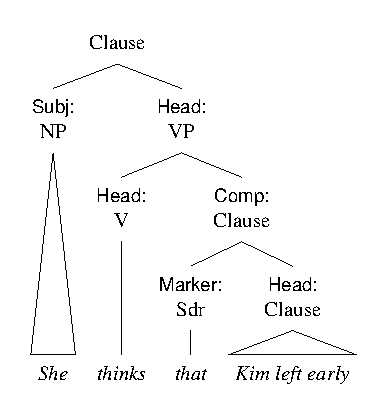
\includegraphics[width=0.55\linewidth]{figures/she thinks that kim left.pdf}
    \caption{Arbre syntaxique montrant la subordination: \mention{that Kim left early} comme complément dans \mention{She thinks that Kim left early}}\label{fig:sub-tree-sub-fr}
\end{figure}

Remarquez que, dans la structure subordonnée, \mention{that} apparaît comme marqueur: il ne projette pas son propre syntagme, mais signale simplement le début de la proposition subordonnée. Un \term{marqueur} (\term{marker}, Mk) est un type de dépendant qui signale comment sa tête se rattache grammaticalement à la structure plus large.

Les propositions de contenu peuvent fonctionner de diverses façons dans la structure plus large:

\ea \label{ex:content-funcs-fr}
    \ea \gll I suspect {\ob}that he left{\cb}.\\
        je soupçonner-PRÉS Sdr il partir-PASSÉ\\
    \glt `Je soupçonne qu'il est parti.' [dans un SV]
    \ex \gll The fact {\ob}that he left{\cb} is clear.\\
        le fait Sdr il partir-PASSÉ être-PRÉS clair\\
    \glt `Le fait qu'il soit parti est clair.' [dans un SN]
    \ex \gll I'm glad {\ob}that he left{\cb}.\\
        je-être content Sdr il partir-PASSÉ\\
    \glt `Je suis content qu'il soit parti.' [dans un SAdj]
    \ex \gll We can proceed provided {\ob}that he left{\cb}.\\
        nous pouvoir-PRÉS continuer pourvu Sdr il partir-PASSÉ\\
    \glt `Nous pouvons continuer pourvu qu'il soit parti.' [dans un SP]
    \ex \gll Whether or not he left is unclear.\\
        si ou non il partir-PASSÉ être-PRÉS peu-clair\\
    \glt `On ne sait pas clairement s'il est parti ou non.' [sujet]
    \ex \gll It's unclear whether or not he left.\\
        il-être peu-clair si ou non il partir-PASSÉ\\
    \glt `Il n'est pas clair s'il est parti ou non.' [sujet extraposé]
    \z
\z

Dans les propositions de contenu déclaratives, le marqueur, c'est-à-dire le subordonnant \mention{that}, peut être obligatoire, facultatif ou inadmissible selon la fonction de la proposition:
\ea\label{ex:marker-need-fr}
    \ea \gll That Kim left surprised no one.\\
        Sdr Kim partir-PASSÉ surprendre-PASSÉ personne\\
    \glt `Que Kim soit partie n'a surpris personne.' [obligatoire]
    \ex \gll I know that Kim left.\\
        je savoir-PRÉS Sdr Kim partir-PASSÉ\\
    \glt `Je sais que Kim est partie.' [facultatif]
    \ex \gll *We left before that Kim arrived.\\
        *nous partir-PASSÉ avant Sdr Kim arriver-PASSÉ\\
    \glt `Sens visé: nous sommes partis avant que Kim arrive. En anglais, \mention{that} est impossible ici.' [*; inadmissible]
\z
\z
Les propositions sujet comme (\ref{ex:marker-need-fr}a) exigent toujours un marqueur. Comme compléments, les déclaratives peuvent le plus souvent apparaître avec ou sans marqueur, comme en (b). La principale exception concerne les cas où elles fonctionnent comme compléments dans des SP, comme en (c).

\label{sec:sub-interrog-fr}

Les propositions de contenu interrogatives sont intéressantes parce qu'elles diffèrent syntaxiquement des interrogatives de proposition principale. Alors que les interrogatives de base en proposition principale peuvent être identifiées par l'inversion sujet--auxiliaire (\mention{Did she accept?}), leurs équivalents subordonnés marquent leur caractère interrogatif avec \mention{whether} ou \mention{if}:

\ea interrogatives de base\label{ex:int-sub-fr}
    \ea \gll Did she accept?\\
        AUX elle accepter\\
    \glt `A-t-elle accepté?' [principale, inversée]
    \ex \gll I wonder {\ob}whether she accepted{\cb}.\\
        je se-demander-PRÉS si elle accepter-PASSÉ\\
    \glt `Je me demande si elle a accepté.' [subordonnée]
    \z
\z
\ea interrogatives focalisées
    \ea \gll How did we get here?\\
        comment AUX nous arriver ici\\
    \glt `Comment sommes-nous arrivés ici?' [principale, inversée]
    \ex \gll I wonder {\ob}how we got here{\cb}.\\
        je se-demander-PRÉS comment nous arriver-PASSÉ ici\\
    \glt `Je me demande comment nous sommes arrivés ici.' [subordonnée]
    \z
\z
Cette distinction est difficile pour les apprenants de l'anglais. Les débutants n'inversent généralement rien et se trompent dans les interrogatives de proposition principale. Les étudiants plus avancés, ayant compris l'inversion, l'appliquent partout et structurent mal les interrogatives subordonnées. Ce n'est qu'à des niveaux beaucoup plus élevés que les étudiants distinguent confortablement les deux.

Cette différence structurale entre interrogatives principales et subordonnées commence toutefois à se défaire, à mesure que l'inversion poursuit sa lente expansion. Même si les propositions de contenu interrogatives inversées restent rares à l'écrit, des exemples comme (\ref{ex:non-inverted-interrogative-fr}) sont devenus assez courants à l'oral. Dans quelques siècles, l'inversion sera peut-être la norme pour toutes les interrogatives et les marqueurs deviendront peut-être facultatifs. Je n'attendrais pas debout.

\ea\label{ex:non-inverted-interrogative-fr}
\gll We need a story of {\ob}how did we get here{\cb}.\\
    nous avoir-besoin-PRÉS une histoire de comment AUX nous arriver ici\\
\glt `Il nous faut une histoire de comment nous sommes arrivés ici.'
\z
Pour l'instant, toutefois, un marqueur, généralement \mention{whether} ou \mention{if}, est toujours obligatoire dans les propositions de contenu interrogatives de base. Sinon, il serait impossible de les distinguer des déclaratives non marquées dans la plupart des cas.

\subsubsection*{Le mandatif}

Un sous-type particulier de construction subordonnée est le \term{mandatif} (\term{mandative}), qui apparaît avec des prédicats exprimant une exigence ou une nécessité:

\ea \label{ex:mandative-fr}
    \ea \gll It is essential {\ob}that he be there{\cb}.\\
        il être-PRÉS essentiel Sdr il être-FORME.NUE là\\
    \glt `Il est essentiel qu'il soit là.' [subjonctif]
    \ex \gll It is essential {\ob}that he should be there{\cb}.\\
        il être-PRÉS essentiel Sdr il should être là\\
    \glt `Il est essentiel qu'il soit là.' [should]
    \ex \gll It is essential {\ob}that he is there{\cb}.\\
        il être-PRÉS essentiel Sdr il être-PRÉS là\\
    \glt `Il est essentiel qu'il est là.' [indicatif]
    \z
\z
La variante au \term{subjonctif} (\term{subjunctive}) utilise la forme nue du verbe, tandis que la variante avec \mention{should} est, ou du moins était, plus courante en anglais britannique. L'anglais américain tend à préférer le subjonctif. La variante à l'\term{indicatif} (\term{indicative}) utilise une forme ordinaire fléchie pour le temps.

C'est un bon exemple de la façon dont les variations dans les propositions subordonnées peuvent porter des nuances de sens et révéler des préférences régionales. Pour l'enseignement, il vaut la peine de noter que la forme indicative devient plus courante, surtout dans les contextes informels, même si le subjonctif reste standard dans l'écrit formel.

\begin{tblsframedsymbol}{Vérifiez votre compréhension: matrice et subordonnée}{test}
Entraînez-vous à identifier les relations structurales:
\begin{itemize}[noitemsep, leftmargin=*]
    \item Dans \mention{I know that she thinks that he left}, identifiez la proposition principale, les propositions matrices et les propositions subordonnées.
    \item Expliquez pourquoi \mention{She asked whether he left} n'a pas d'inversion, alors que \mention{Did he leave?} en a une.
    \item Trouvez la structure mandative: \mention{It's important that he be careful} par opposition à \mention{It's important that he is careful}.
\end{itemize}
Comprendre ces relations structurales aide à voir comment le sens émerge de l'architecture syntaxique.
\end{tblsframedsymbol}

\subsection{Propositions comparatives}

Le deuxième grand type de proposition subordonnée finie est la proposition comparative. Ces propositions complètent une comparaison, comme dans (\ref{ex:comparative-intro-fr}).

\ea \label{ex:comparative-intro-fr}
    \ea \gll The ice was thicker than {\ob}we expected{\cb}.\\
        la glace être-PASSÉ plus-épaisse que nous attendre-PASSÉ\\
    \glt `La glace était plus épaisse que nous ne l'avions prévu.'
    \ex \gll She writes faster than {\ob}she speaks{\cb}.\\
        elle écrire-PRÉS plus-vite que elle parler-PRÉS\\
    \glt `Elle écrit plus vite qu'elle ne parle.'
    \ex \gll It doesn't cost as much as {\ob}I'd thought{\cb}.\\
        cela NEG coûter-PRÉS autant que je-avoir-PASSÉ penser\\
    \glt `Cela ne coûte pas autant que je l'avais pensé.'
    \z
\z
Ce qui distingue les comparatives des propositions de contenu, c'est qu'elles comportent de l'ellipse: des éléments récupérables à partir du contexte sont laissés de côté. Dans (\ref{ex:comparative-ellipsis-fr}), les points de suspension indiquent cette ellipse.\footnote{Dans un chapitre précédent, j'ai introduit les lacunes. Les lacunes diffèrent de l'ellipse: ce sont des éléments structuraux dans les arbres; l'ellipse est du matériau récupérable sémantiquement dans le contexte, mais non présent comme élément syntaxique.}

\ea \label{ex:comparative-ellipsis-fr}
    \ea \gll Kim read more books than {\ob}Pat read \dots{\cb}.\\
        Kim lire-PASSÉ plus livres que Pat lire-PASSÉ \dots\\
    \glt `Kim a lu plus de livres que Pat n'en a lu.'
    \ex \gll Kim read more books than {\ob}Pat did \dots{\cb}.\\
        Kim lire-PASSÉ plus livres que Pat AUX.PASSÉ \dots\\
    \glt `Kim a lu plus de livres que Pat.'
    \ex \gll Kim read more books than {\ob}Pat{\cb}.\\
        Kim lire-PASSÉ plus livres que Pat\\
    \glt `Kim a lu plus de livres que Pat.'
    \z
\z

Les deux premières variantes montrent l'ellipse; en (b), la proforme \mention{did} remplace la répétition de \mention{read}. La troisième, (c), contient \mention{Pat} comme complément de SN plutôt que comme complément propositionnel. Les trois signifient essentiellement la même chose.

Contrairement à la plupart des cas d'ellipse, dans les comparatives il est agrammatical de fournir l'information omise: *\mention{Kim read more books than Pat read 20 books} ou *\mention{It's not as deep as it is 20 cm wide}. L'ellipse est une partie centrale de ce type de proposition. La structure de la proposition comparative est montrée dans la figure~\ref{fig:comp-tree-fr}.

\begin{figure}
    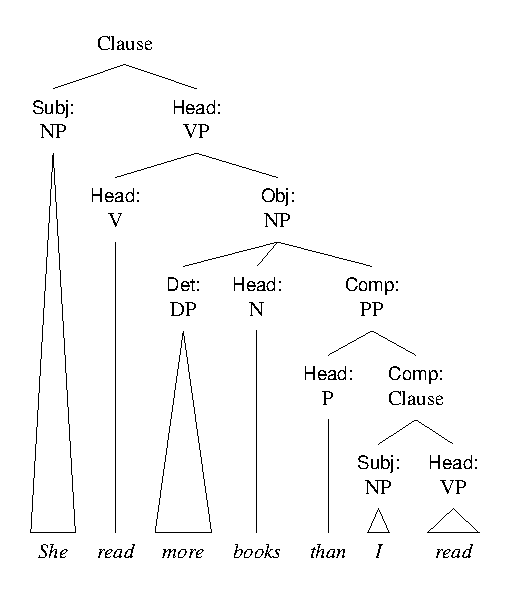
\includegraphics[width=0.7\linewidth]{figures/she read more books than I read.pdf}
    \caption{Arbre syntaxique montrant une proposition comparative avec ellipse}\label{fig:comp-tree-fr}
\end{figure}

Les propositions comparatives fonctionnent comme compléments dans un SP en \mention{than} ou en \mention{as}, selon le type de comparaison exprimé.

\ea \label{ex:comp-markers-fr}
    \ea \gll Kim is taller than {\ob}Pat is{\cb}.\\
        Kim être-PRÉS plus-grand que Pat être-PRÉS\\
    \glt `Kim est plus grande que Pat.' [inégalité]
    \ex \gll Kim is as tall as {\ob}Pat is{\cb}.\\
        Kim être-PRÉS aussi grand que Pat être-PRÉS\\
    \glt `Kim est aussi grande que Pat.' [égalité\footnote{Le terme \emph{égalité} peut être légèrement trompeur ici. L'exemple signifie que Kim est au moins aussi grande que Pat; elle peut même être plus grande.}]
    \z
\z
\mention{Than} en (\ref{ex:comp-markers-fr}a) signale l'inégalité, tandis que \mention{as} en (b) marque l'égalité. Le premier \mention{as} est un adverbe: nous avons le SAdj \mention{as tall}, avec \mention{as} comme modificateur. Le second est une préposition.

Pour les apprenants de l'anglais, les propositions comparatives posent plusieurs difficultés:
\begin{itemize}[noitemsep]
    \item comprendre quand on peut omettre du matériau et quelle quantité on peut omettre;
    \item maîtriser les différents schémas de l'égalité et de l'inégalité;
    \item traiter des comparaisons complexes qui comportent plusieurs éléments.
\end{itemize}

La bonne nouvelle est que les comparatives suivent des schémas assez réguliers. Les apprenants peuvent généralement maîtriser les formes de base, comme \mention{taller than} `plus grand que' et \mention{as tall as} `au moins aussi grand que', avant d'aborder des structures plus complexes.

\section{Coordination}\label{sec:coordination-fr}

Alors que la subordination crée des relations de dépendance entre propositions, la \term{coordination} unit des éléments de même statut syntaxique. Au centre de ce système se trouve une petite classe fermée de mots, les \term{coordonnants} (\term{coordinators}, Crd), principalement \mention{and}, \mention{or} et \mention{but} (il faut les trois rien que pour les énumérer). Comme les subordonnants, les coordonnants fonctionnent comme marqueurs.

Attention au mot français \term{coordination}: il ne désigne pas simplement le fait que deux idées se suivent bien dans le discours. Ici, il s'agit d'une relation structurale précise: deux éléments ont le même statut syntaxique et aucun des deux ne gouverne l'autre comme tête.

Considérez ces exemples:

\ea \label{ex:coord-basic-fr}
    \ea \gll {\ob}Jane is a good teacher{\cb} {\ob}and her students really like her{\cb}.\\
        Jane être-PRÉS une bonne enseignante et ses étudiants vraiment aimer-PRÉS elle\\
    \glt `Jane est une bonne enseignante et ses étudiants l'aiment vraiment.'
    \ex \gll They offered us a choice of {\ob}red wine{\cb}, {\ob}white wine{\cb}, {\ob}or beer{\cb}.\\
        ils offrir-PASSÉ nous un choix de rouge vin blanc vin ou bière\\
    \glt `Ils nous ont offert le choix entre du vin rouge, du vin blanc ou de la bière.'
    \ex \gll Her assistant is {\ob}very young{\cb} {\ob}but a quick learner{\cb}.\\
        son assistant être-PRÉS très jeune mais un rapide apprenant\\
    \glt `Son assistante est très jeune mais apprend vite.'
    \z
\z
Les éléments entre crochets dans ces exemples fonctionnent comme \term{coordonnés} (\term{coordinates}). Cette fonction peut être réalisée par des propositions, comme dans (\ref{ex:coord-basic-fr}a), par des SN ou d'autres syntagmes, comme en (b), ou, plus rarement, par un mélange de catégories comme le SAdj et le SN en (c). Les coordonnants expriment généralement des relations distinctes: \mention{and} pour l'addition, \mention{or} pour l'alternative et \mention{but} pour le contraste.

Ce qui distingue la coordination des constructions vues auparavant, c'est qu'elle est sans tête: aucun coordonné n'est la tête de l'ensemble. Cette absence de tête se voit dans un test simple. Dans la plupart des cas, on peut remplacer toute la coordination par l'un ou l'autre de ses coordonnés:

\ea \label{ex:coord-replace-fr}
    \ea \gll Her assistant is very young.\\
        son assistant être-PRÉS très jeune\\
    \glt `Son assistante est très jeune.'
    \ex \gll Her assistant is a quick learner.\\
        son assistant être-PRÉS un rapide apprenant\\
    \glt `Son assistante apprend vite.'
    \z
\z
(\ref{ex:coord-replace-fr}a) et (b) sont deux alternatives grammaticales à (\ref{ex:coord-basic-fr}c). C'est très différent des constructions à tête comme \mention{very young}, où l'on peut utiliser la tête seule (\mention{she's young}), mais pas le dépendant seul (*\mention{she's very}). La structure de coordination est montrée dans la figure~\ref{fig:coord-basic-fr}.

\begin{figure}
    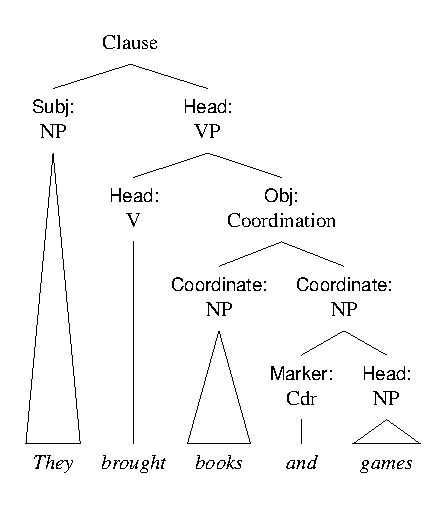
\includegraphics[width=0.65\linewidth]{figures/the brought books and games.pdf}
    \caption{Coordination de base avec marqueur: \mention{They brought books and games}}\label{fig:coord-basic-fr}
\end{figure}

\subsection{Propriétés de la coordination}

Trois propriétés principales distinguent la coordination des autres constructions.

Il n'y a pas de limite grammaticale au nombre de coordonnés, sauf avec \mention{but}:

\ea \label{ex:coord-multiple-fr}
\gll Nothing noble, sublime, profound, delicate, tasteful or even decent can find a place.\\
    rien noble sublime profond délicat de-bon-goût ou même convenable pouvoir-PRÉS trouver une place\\
\glt `Rien de noble, sublime, profond, délicat, de bon goût ou même convenable ne peut trouver place.'
\z

Les coordonnés doivent être fonctionnellement semblables: ils doivent pouvoir remplir la même fonction s'ils sont utilisés seuls.

\ea \label{ex:coordinate-function-fr}
    \ea \gll I'll be back next week or at the end of the month.\\
        je-FUT être de-retour semaine prochaine ou à la fin du mois\\
    \glt `Je serai de retour la semaine prochaine ou à la fin du mois.' [ajoints temporels]
    \ex \gll *We're leaving Rome and next week.\\
        *nous partir-PRÉS Rome et semaine prochaine\\
    \glt `Structure visée impossible en anglais: \mention{Rome} est objet, mais \mention{next week} est ajoint.' [*; objet et ajoint]
    \z
\z

Un coordonné étendu, c'est-à-dire un coordonné accompagné de son coordonnant, ne peut jamais être déplacé au début:

\ea \label{ex:coord-front-fr}
    \ea \gll They attended but they aren't members.\\
        ils assister-PASSÉ mais ils NEG-être-PRÉS membres\\
    \glt `Ils ont assisté à la réunion, mais ils ne sont pas membres.'
    \ex \gll *But they aren't members, they attended.\\
        *mais ils NEG-être-PRÉS membres ils assister-PASSÉ\\
    \glt `Sens visé: ils ont assisté à la réunion, mais ils ne sont pas membres. En anglais, le coordonné étendu avec \mention{but} ne peut pas être placé ainsi au début.' [*]
    \z
\z

\subsection{Remarque sur les coordonnants en début de phrase}

Une règle prescriptive déconseille de commencer une phrase par des coordonnants comme \mention{and} ou \mention{but}. Cette interdiction n'a aucun fondement dans la grammaire ou l'usage de l'anglais. Des écrivains habiles ont utilisé des coordonnants en début de phrase tout au long de l'histoire de l'anglais, y compris dans ce livre; vous en trouverez de nombreux exemples dans ce chapitre et ailleurs. Toutefois, un coordonnant en début de phrase ne peut pas unir sa phrase à la précédente dans une coordination étroite: rappelez-vous la restriction sur l'antéposition dans (\ref{ex:coord-front-fr}). Il peut plutôt fonctionner comme \term{connecteur discursif} (\term{discourse connector}), en signalant la relation entre la nouvelle phrase et ce qui précède.

Cette distinction est importante en français aussi: un connecteur discursif relie des morceaux de texte, tandis qu'une coordination syntaxique relie des éléments dans une même structure. Le seul vrai frein est stylistique: comme tout procédé, les coordonnants en début de phrase peuvent devenir monotones s'ils sont trop fréquents. Employés avec mesure, ils sont utiles pour gérer le fil du discours et signaler les relations textuelles.

\subsection{Types de coordination}

La distinction la plus simple oppose la \term{coordination symétrique} (\term{symmetric coordination}), où l'ordre des coordonnés ne change pas le sens, et la \term{coordination asymétrique} (\term{asymmetric coordination}), où l'ordre compte:

\ea \label{ex:coord-sym-fr}
    \ea \gll I was hungry and tired.\\
        je être-PASSÉ faim et fatigué\\
    \glt `J'avais faim et j'étais fatigué.' [symétrique]
    \ex \gll I got up and had breakfast.\\
        je lever-PASSÉ et prendre-PASSÉ petit-déjeuner\\
    \glt `Je me suis levé et j'ai pris le petit-déjeuner.' [asymétrique]
    \z
\z
Dans (\ref{ex:coord-sym-fr}a), inverser les coordonnés ne change pas le sens. Mais dans (b), l'ordre implique une séquence: se lever a eu lieu avant le petit-déjeuner.

On distingue aussi la \term{coordination distributive} (\term{distributive coordination}) de la \term{coordination conjointe} (\term{joint coordination}):

\ea \label{ex:coord-dist-fr}
    \ea \gll Kim and Pat are fine players.\\
        Kim et Pat être-PRÉS bons joueurs\\
    \glt `Kim et Pat sont de bons joueurs.' [distributive]
    \ex \gll Kim and Pat are a good pair.\\
        Kim et Pat être-PRÉS une bonne paire\\
    \glt `Kim et Pat forment une bonne paire.' [conjointe]
    \z
\z
Dans (\ref{ex:coord-dist-fr}a), la propriété d'être un bon joueur s'applique à Kim et à Pat individuellement. Mais dans (b), former une bonne paire ne peut s'appliquer qu'aux deux ensemble; aucun des deux ne pourrait être une paire à lui seul.

\subsection{Marquage de la coordination}

La coordination peut être marquée de plusieurs façons:
\begin{itemize}[noitemsep]
    \item Avec un coordonnant: \mention{red and blue}
    \item Sans aucun marqueur: \mention{red, white, blue}
    \item Avec des coordonnants répétés: \mention{red or white or blue}
    \item Avec des marqueurs corrélatifs: \mention{both red and blue}
\end{itemize}

Même si les coordonnants expriment typiquement l'addition (\mention{and}), l'alternative (\mention{or}) et le contraste (\mention{but}), ils peuvent porter des significations supplémentaires en coordination asymétrique:

\ea \label{ex:coord-meaning-fr}
    \ea \gll Pay within a week and you'll get a discount.\\
        payer dans une semaine et tu-FUT obtenir une réduction\\
    \glt `Paie dans la semaine et tu obtiendras une réduction.' [conditionnelle]
    \ex \gll Pay within a week or you'll lose the discount.\\
        payer dans une semaine ou tu-FUT perdre la réduction\\
    \glt `Paie dans la semaine, sinon tu perdras la réduction.' [conditionnelle négative]
    \z
\z

\begin{tblsframedsymbol}{Reconnaissance de schémas: coordination ou subordination?}{test}
Appliquez les diagnostics pour distinguer ces structures:
\begin{itemize}[noitemsep, leftmargin=*]
    \item \mention{She thinks that he left} et \mention{She left and he stayed}: quel exemple insère une proposition dans une autre, et lequel unit deux propositions de statut égal?
    \item \mention{Although it rained, we went} et \mention{It rained but we went}: lequel montre une hiérarchie de dépendance, et lequel montre un statut égal?
    \item \mention{*But we went, it rained} et \mention{Although it rained, we went}: que révèle l'antéposition sur la structure?
\end{itemize}
Ces tests aident à distinguer l'enchâssement hiérarchique de l'union entre éléments de statut égal.
\end{tblsframedsymbol}

Avec l'introduction des coordonnants, nous avons maintenant rencontré toutes les grandes catégories lexicales de l'anglais sauf les interjections, ainsi que les principales fonctions syntaxiques qu'elles remplissent dans les propositions.

\subsection{Structure de la coordination}

Quand nous coordonnons des éléments, ils doivent partager la même fonction syntaxique. On peut donc coordonner des compléments avec des compléments ou des modificateurs avec des modificateurs, mais pas un complément avec un modificateur. Comparez:

\ea \label{ex:coord-function-fr}
    \ea \gll We listened {\ob}to the teacher{\cb} {\ob}and the students{\cb}.\\
        nous écouter-PASSÉ à le professeur et les étudiants\\
    \glt `Nous avons écouté le professeur et les étudiants.' [compléments]
    \ex \gll We listened {\ob}Monday{\cb} and {\ob}Tuesday{\cb}.\\
        nous écouter-PASSÉ lundi et mardi\\
    \glt `Nous avons écouté lundi et mardi.' [modificateurs]
    \ex \gll *We listened {\ob}to the teachers{\cb} and {\ob}Monday{\cb}.\\
        *nous écouter-PASSÉ à les professeurs et lundi\\
    \glt `Structure visée impossible en anglais: \mention{to the teachers} est complément, mais \mention{Monday} est modificateur.' [*; fonctions mixtes]
    \z
\z
Les éléments coordonnés, appelés \term{coordonnés}, peuvent provenir de n'importe quel grand type de syntagme: noms, verbes, adjectifs, prépositions, syntagmes plus larges ou propositions. Ce qui compte, c'est qu'ils fonctionnent de la même façon dans la structure plus large.

\subsection{Coordination avec et sans marqueurs}

La coordination peut apparaître avec ou sans coordonnant explicite. Quand il n'y a pas de coordonnant, on parle de \term{coordination asyndétique} (\term{asyndetic coordination}):

\ea \label{ex:coord-marking-fr}
    \ea \gll She brought {\ob}games{\cb}, {\ob}stories{\cb}, {\ob}songs{\cb}.\\
        elle apporter-PASSÉ jeux histoires chansons\\
    \glt `Elle a apporté des jeux, des histoires, des chansons.' [asyndétique]
    \ex \gll She brought {\ob}games{\cb}, {\ob}stories{\cb}, and {\ob}songs{\cb}.\\
        elle apporter-PASSÉ jeux histoires et chansons\\
    \glt `Elle a apporté des jeux, des histoires et des chansons.' [syndétique]
    \z
\z
En plus de la coordination simple avec un seul coordonnant, nous pouvons avoir une \term{coordination corrélative} (\term{correlative coordination}), où des marqueurs apparaissent avec plusieurs coordonnés:

\ea \label{ex:coord-correlative-fr}
    \ea \gll {\ob}Both{\cb} tired {\ob}and{\cb} hungry\\
        à-la-fois fatigué et affamé\\
    \glt `À la fois fatigué et affamé'
    \ex \gll {\ob}Either{\cb} now {\ob}or{\cb} never\\
        soit maintenant soit jamais\\
    \glt `Soit maintenant, soit jamais'
    \ex \gll {\ob}Neither{\cb} simple {\ob}nor{\cb} easy\\
        ni simple ni facile\\
    \glt `Ni simple ni facile'
    \z
\z

\subsection{Coordination à plusieurs niveaux}

Il arrive que les coordonnés contiennent eux-mêmes une coordination; c'est ce que nous appelons une coordination à plusieurs niveaux. Considérez cet exemple:

\ea \label{ex:coord-layered-fr}
\gll The story was {\ob}short and sweet{\cb} but {\ob}complex and thought-provoking{\cb}.\\
    l'histoire être-PASSÉ courte et douce mais complexe et stimulante\\
\glt `L'histoire était courte et charmante, mais complexe et stimulante.'
\z
Ici, nous avons deux coordonnés principaux reliés par \mention{but}, mais chacun de ces coordonnés contient sa propre coordination interne avec \mention{and}. Cette superposition permet d'exprimer des relations complexes entre idées tout en gardant une structure claire. La structure à plusieurs niveaux est montrée dans la figure~\ref{fig:coord-layered-fr}.

\begin{figure}
    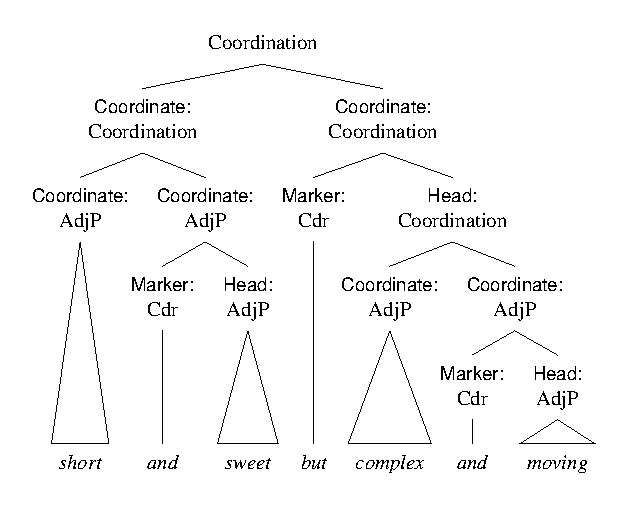
\includegraphics[width=0.9\linewidth]{figures/short and sweet but complex and moving.pdf}
    \caption{Coordination à plusieurs niveaux: \mention{short and sweet but complex and moving}}\label{fig:coord-layered-fr}
\end{figure}

\subsection{Types particuliers de coordination}

Un type de coordination particulièrement intéressant apparaît dans les structures comparatives:

\ea \label{ex:coord-comp-fr}
    \ea \gll He's as tall as {\ob}or taller than{\cb} his brother.\\
        il-être aussi grand que ou plus-grand que son frère\\
    \glt `Il est aussi grand que son frère, ou plus grand que lui.'
    \ex \gll She writes more {\ob}but understands less{\cb} than before.\\
        elle écrire-PRÉS plus mais comprendre-PRÉS moins que avant\\
    \glt `Elle écrit davantage mais comprend moins qu'avant.'
    \z
\z
Ces structures comportent souvent des relations complexes entre les coordonnés et les éléments qu'ils partagent. Leur interprétation exige de comprendre à la fois la coordination et la relation comparative.

\begin{tblsframedsymbol}{Auto-vérification rapide: structures complexes}{test}
Testez votre capacité à analyser des structures à plusieurs niveaux:
\begin{itemize}[noitemsep, leftmargin=*]
    \item Dans \mention{I know that she left and he stayed}, identifiez toutes les relations de subordination et de coordination.
    \item Dans \mention{Both young and talented, she succeeded}, identifiez les marqueurs corrélatifs et les adjectifs coordonnés.
    \item Analysez la structure suivante: \mention{He's taller than I thought but shorter than his brother}.
\end{itemize}
Comprendre ces schémas complexes aide à voir comment la subordination et la coordination travaillent ensemble pour construire le sens.
\end{tblsframedsymbol}

\section{Résumé}

La subordination et la coordination font le même travail, relier des idées, mais avec des architectures opposées. La subordination enchâsse; la coordination unit. Une bonne écriture équilibre les deux. Quand vous pouvez reconnaître la structure vers laquelle un étudiant se dirige et l'endroit où elle se dérègle, vous pouvez nommer le problème: trop de couches, trop d'énumération, ou un subordonnant là où un coordonnant suffirait, au lieu de simplement sentir que quelque chose ne va pas.
